\documentclass{report}

\usepackage{a4}
\usepackage[hypertex]{hyperref}
\usepackage{graphicx}

\begin{document}

\title{Exploring Machine Learning:\\
  The ID3 algorithm}

\author{Mohammed Ibrahim\\
 Computer Science Department\\
  College of Science, Swansea University\\
  Swansea, SA2 8PP, UK
}

\maketitle

\tableofcontents

\chapter{File Format}
\label{sec:fileformat}

\section{File Format}
\label{sec:file}

A file format is a specific way that information is encoded for storage in a computer file. There are different kinds of file formats for different kinds of information. Some file formats are designed for very particular sorts of data.

The file format which I have decided so far:

\begin{itemize}

\item The program ignore the first line in a file as comment.
\item The program read the second line that is attributes.
\item The program splits the words explicitly and it use the space and commas to read the possible values. 

The syntax : 

\item Line 1 : Comment: The program ignores.
\item Line 2 : attribute(1), attribute(2), attribute(n). The program will read the number of attributes in a single row.
\item Line 3 : The program reads the possible values.
\item Line n : The program reads the number of possible values.

\end{itemize}


The another choice is to use the Backus–Naur Form (BNF) is one of the two main notion techniques for context-free grammars, often used to describe the syntax of languages used in computing, such as computer programming language, document formats, instruction sets and communication protocol.





\section{Comma-separated values}
\label{sec:csv}

To refer from \cite{Wikipedia_CommaSeparatedValues}(page 1): A comma-separated values(CSV) file stores tabular data(numbers and text)in plain text form. Plain text means that the file is a sequence of characters, with no data that has to be interpreted instead, as binary numbers. A CSV file consists of any number of records, separated by line breaks of some kind; each record consists of fields, separated by some other character or string, most commonly a literal TAB or comma. Usually, all records have an identical sequence of fields.


\section{Identifiers}
\label{sec:ide}

According to \cite{Roberts2000CompleteJava2Certification}(Chapter 1, page 6): An identifier is a name used by a programmer to variable, method, package, class, interfaces or label. Keywords and reserved words can't be used as  identifiers. It must begin with a letter, a dollar sign, or an underscore; identifiers are case sensitive. Identifiers are tokens (also called symbols) which name as language entities. Each variable has a name by which it is identified in the program.

\section{Decision Tree}
According to \cite{Mitchell1997MachineLearning}(page 59,Chapter 3): Training set : In machine learning training sets are generally called as tables, where each row in the table represents a single training example. 

To illustrate the operation of ID3, we consider the learning task represented by the example training set given in Figure \ref{fig:trainingplaytennis}. We have four attributes Outlook, Temperature, Humidity and Wind. The target attribute is called PlayTennis, which has values boolean value \texttt{yes} or \texttt{no} for different Saturday mornings, is to be predicted based on other attributes of the morning in question.
\begin{figure}[h]
  \centering
  \begin{tabular}{|c|l|l|l|l|l|l|}
    \hline
    Day & Outlook & Temperature & Humidity & Wind & PlayTennis\\
    \hline
    1 & sunny & hot & high & weak & no
    \\\hline
    2 & sunny & hot & high & strong & no
    \\\hline
    3 & overcast & hot & high & weak & yes
    \\\hline
    4 & rain & mild & high & weak & yes
    \\\hline
    5 & rain & cool & normal & weak & yes
    \\\hline
    6 & rain & cool & normal & strong & no
    \\\hline
    7 & overcast & cool & normal & strong & yes
    \\\hline
    8 & sunny & mild & high & weak & no
    \\\hline
    9 & sunny & cool & normal & weak & yes
    \\\hline
    10 & rain & mild & normal & weak & yes
    \\\hline
    11 & sunny & mild & normal & strong & yes
    \\\hline
    12 & overcast & mild & high & strong & yes
    \\\hline
    13 & overcast & hot & normal & weak & yes
    \\\hline
    14 & rain & mild & high & strong & no
    \\\hline
  \end{tabular}
  \caption{Training set for \texttt{PlayTennis} example}
  \label{fig:trainingplaytennis}
\end{figure}

The below figure shows the complete decision tree for the above training set.\ref{fig:decisiontree}

\begin{figure}[h]
\centering
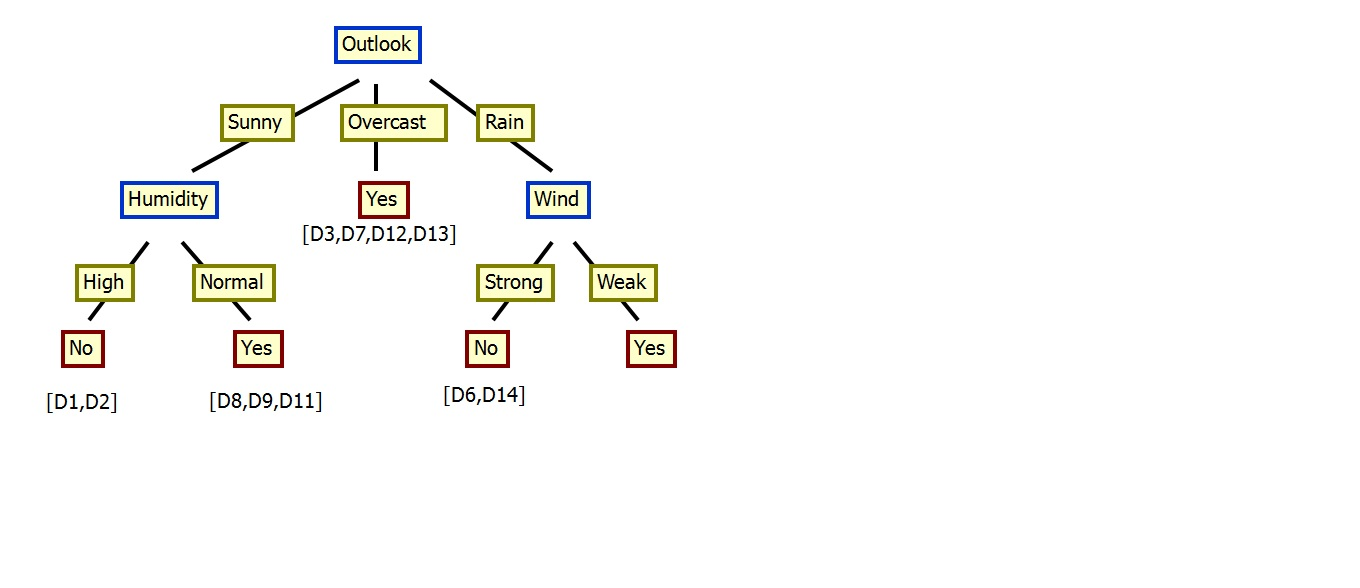
\includegraphics[bb=0 0 1360 588,scale=0.5,keepaspectratio=true]{DecisionTree.jpg}
\caption{Decision Tree}
\label{fig:decisiontree}
\end{figure}


\begin{figure}[h]
  \centering
  \begin{tabular}{|c|l|l|l|l|l|l|}
    \hline
   Slno & Skin	& Colour & Size & Flesh & Conclusion\\
    \hline
    1 & hairy &	brown &	large &	hard & safe	
    \\\hline
    2 & hairy & green & large & hard & safe
    \\\hline
    3 & smooth & red & large & soft & dangerous
    \\\hline
    4 & hairy & green & large & soft & safe	
    \\\hline
    5 & hairy &	red & small	& hard	& safe
    \\\hline
    6 & smooth & red & small & hard & safe	
    \\\hline
    7 & smooth & brown & small & hard &	safe	
    \\\hline
    8 & hairy &	green &	small &	soft & dangerous	
    \\\hline
    9 & smooth & green & small & hard &	dangerous
    \\\hline
    10 & hairy & red & large & hard & safe
    \\\hline
    11 & smooth & brown & large & soft & safe	
    \\\hline
    12 & smooth	& green & small	& soft	& dangerous
    \\\hline
    13 & hairy	& red & small & soft & safe	
    \\\hline
    14 & smooth	& red &	large &	hard & dangerous
    \\\hline
    15 & smooth & red & small &	hard & safe
    \\\hline
    16 & hairy & green & small & hard & dangerous		
    \\\hline
                 
    
  \end{tabular}
  \caption{Training set for \texttt{FoodExample} example}
  \label{fig:foodexample}
\end{figure}



\begin{figure}[h]
  \centering
  \begin{tabular}{|c|l|l|l|l|l|l|}
    \hline
    AGE & COMPETITION & TYPE & PROFIT\\
    \hline
    old	& yes & software & down
    \\\hline
    old & no & software & down
    \\\hline
    old	& no & hardware & down
    \\\hline
   	mid	& yes & software & down
    \\\hline
    mid	& yes & hardware & down
    \\\hline
    mid & no & hardware & up
    \\\hline
    mid & no & software & up
    \\\hline
    new & yes & software & up
    \\\hline
    new & no & hardware	& up
	\\\hline
	new	& no & software	& up
	\\\hline
   
  \end{tabular}
  \caption{Training set for \texttt{StockExample} example}
  \label{fig:stockexample}
\end{figure}





\bibliographystyle{plain}
\bibliography{Bibliography}



\end{document}